\subsection{Experimentación}
Para la experimentación llevada a cabo, hay dos categorias principales. La primera platea experimentos $``$genericos", entendidos como experimentos donde no hubo mucha lógica detrás de ellos. La segunda es la categoria de casos favorables para uno u otro algoritmo. Ambas categorias son explicadas en detalle en su respectiva sección.

En los dos casos, la cantidad de $`$n' nodos era 10 $\leq$ $n$ $\leq$ 800, incrementando el valor de $`$n' en 10 para cada salto. Se realizaron 5 ejecuciones para cada juego de datos y se tomo el promedio de las mismas para representarlo en el gráfico.

No se tomaron casos de $`$n' mayor a 800 ya que el tiempo de ejecución de los mismos ponía en peligro la presentación del trabajo práctico.

\subsubsection{Experimento genérico} \label{generico}
En el caso de los experimentos genericos, los mismos fueron desarrollados bajo los siguientes casos: una instancia sin arbitraje, otra con un único ciclo de arbitraje de longitud variable.

Tal como fue mencionado en la introducción, estos casos fueron diseñados sin mucha lógica detras. Qué significa esto? Significa que en el caso sin arbitraje solo se completó la matriz de tipos de cambio con elementos menores a 1 para cada $`$i', $`$j' en la matriz, excepto por la diagonal que contiene 1s. En el caso del único ciclo de longitud variable, se inicializa la matriz con todos valores cercanos a 0, excepto por la diagonal, y luego se cambia una cantidad aleatoria de los elementos cercanos a 0 a un valor un poco mayor a 1, por último, se cambia el valor de un nodo a 2.

\subsubsubsection{Sin Arbitraje} \label{sinArbitraje}
Como fue explicado arriba, para este experimento se generó una matriz con valores menores que 1, para que no haya arbitraje. Dadas las complejidades temporales de los algoritmos, se espera en este caso que el tiempo de ejecución sea parecido para ambos algoritmos. Esto principalmente se espera así ya que Bellman-Ford, en cualquier escenario, debe terminar de recorrer el grafo para poder terminar la ejecución. En cambio, el algoritmo de Floyd interrumpe su ejecución al encontrar un ciclo que cumpla. Como no hay arbitraje, ambos algoritmos deben recorrer todos los puntos del grafo.

\begin{figure}[H]
  \begin{center}
	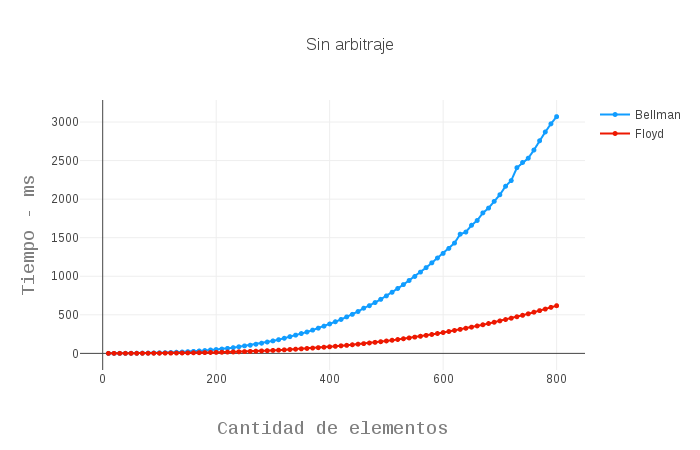
\includegraphics[scale=0.4]{images/experimentos/arbitraje/sinArbitraje.png}
  \end{center}
\end{figure}

La ejecución no se comporta como fue esperado ya que la diferencia de tiempos entre los dos algoritmos es bastante amplia. Es probable que haya alguna implementación dentro del algoritmo de Bellman-Ford que esté causando la diferencia de tiempos. Sin embargo, si se puede observar que la curva es creciente en ambos casos, lo cual implica que siempre se fue cumpliendo con el peor caso.


\subsubsubsection{Único Ciclo de Longitud Variable} \label{unicoCiclo}
Dado que en escencia, la matriz presentada en este caso es muy parecida al caso anterior, se espera una ejecución parecida. Recordamos que la diferencia con la matriz anterior es que esta contiene un ciclo de arbitraje.

Es por ello, que sabiendo que Floyd puede finalizar su ejecución antes si encuentra el ciclo de arbitraje, es posible que la ejecución del mismo sea más rapida que en el caso anterior.

\begin{figure}[H]
  \begin{center}
	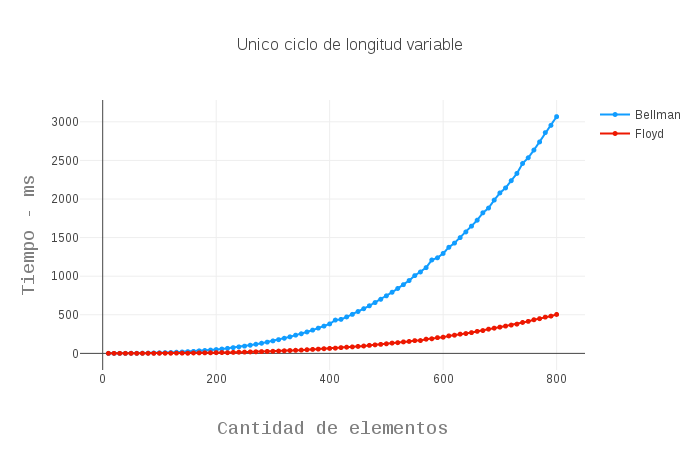
\includegraphics[scale=0.4]{images/experimentos/arbitraje/unicoCicloLongitudVariable.png}
  \end{center}
\end{figure}

Como era de esperar, la ejecución de ambos algoritmos es parecida al caso anterior, pero con una leve mejora en el caso de Floyd. Es importante tener en cuenta que esta mejora es leve porque existe un único ciclo que puede tener longitud $`$n', lo cual implica que no necesariamente vaya a ser rapidamente encontrado por el algoritmo.

\subsubsection{Experimento Favorables por Algoritmo} \label{favorables}

Para esta categoria se generaron dos instancias principales, una donde la matriz favorezca a Bellman-Ford y la otra que favorezca a Floyd-Warshall.

\subsubsubsection{Favorable Bellman-Ford} \label{favorableBellmanFord}
El caso favorable a Bellman-Ford es aquel en donde no hay arbitraje y algoritmo pudo finalizar su ejecución antes de recorrer toda la matriz. Recordemos que Bellman-Ford finaliza su ejecución cuando termina de relajar todas sus aristas. Recordemos que el que haya arbitraje es equivalente a que haya un ciclo negativo, dicho ciclo se encontraría al iterar $`$n' veces. Es por ello que como no hay arbitraje, es probable que no sea necesario iterar el grafo por completo, logrando así en teoria una mejor ejecucion temporal que Floyd-Warshall. Este ultimo algoritmo finaliza antes su ejecución si encuentra un ciclo negativo, que en este caso no existe.

Sin embargo, si tenemos en cuenta el resultado del primer experimento, el cual es muy parecido a este, es probable que la ejecución de Floyd-Warshall sea mejor que la de Bellman-Ford.

\begin{figure}[H]
  \begin{center}
	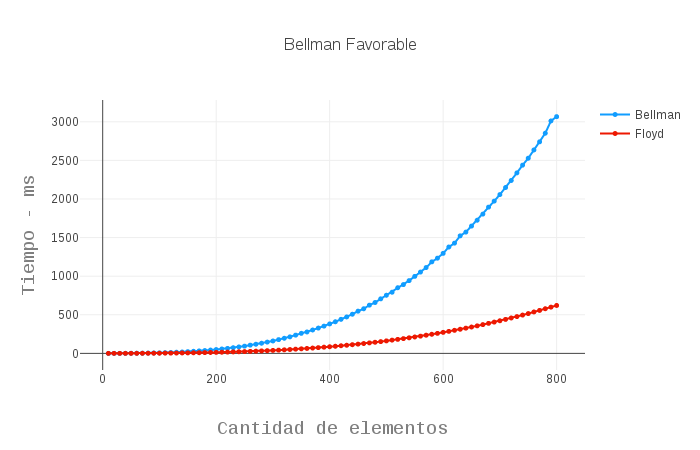
\includegraphics[scale=0.4]{images/experimentos/arbitraje/bellmanFavorable.png}
  \end{center}
\end{figure}

Tal como era de suponer, la ejecución de Floyd-Warshall es mucho mejor que la de Bellman-Ford. Esto llama la atención especialmente por lo mencionado arriba, donde este es un caso en el que Bellman-Ford fue claramente favorecido. Nuevamente, es probablemente que haya alguna implementación en el algoritmo que no permita llegar a la complejidad temporal esperada.

\subsubsubsection{Favorable Floyd-Warshall} \label{favorableFloydWarshall}
Para favorecer la ejecución de Floyd-Warshall, se busco que las instancias a ejecutar contengan un ciclo de arbitraje y que el mismo se encuentre en la primera parte de la matriz, en particular entre los primeros n/4 elementos. De esta manera, es más visible la comparación contra Bellman-Ford dado que este debe ejecutarse por completo y Floyd-Warshall finalizará su ejecución al recorrer los primeros n/4 elementos.

\begin{figure}[H]
  \begin{center}
	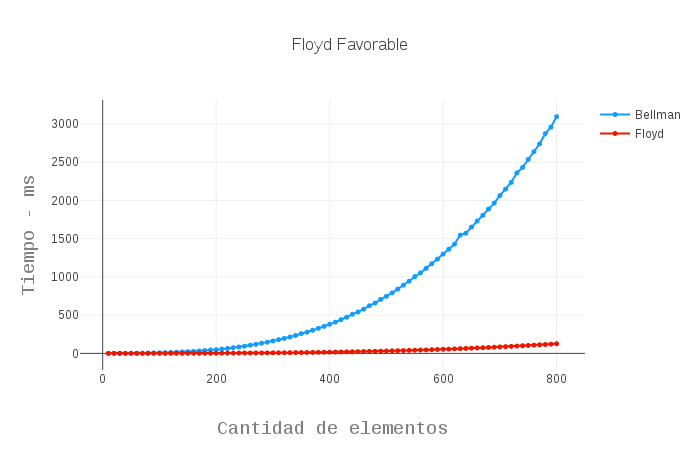
\includegraphics[scale=0.4]{images/experimentos/arbitraje/floydFavorable.png}
  \end{center}
\end{figure}

Como se puede observar en el grafico, la diferencia de tiempos es muy grande. Recordamos que la ejecución de Bellman-Ford es probable que no sea consistente con su cota teorica, como dijimos en los experimentos anteriores. Sin embargo hay una gran diferencia entre la ejecución de uno y otro algoritmo.